\begin{frame}{Distance-dependent connectivity in anisotropic networks}
  % 
  \begin{columns}
    % 
    \begin{column}{.45\textwidth}
      \begin{figure}
        \centering
        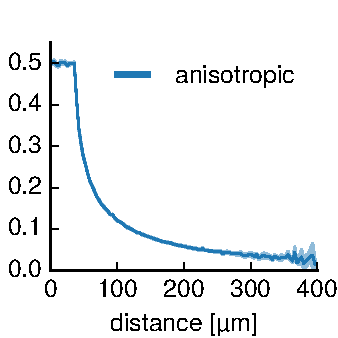
\includegraphics[width=0.85\textwidth]{%
          figures/netw_dist-dep_aniso.pdf} %
      \end{figure}


    \end{column}
    % 
    \begin{column}{.55\textwidth}
      \begin{figure}
        \centering
        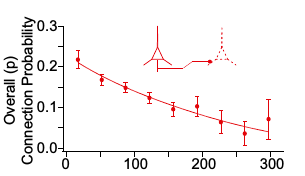
\includegraphics[width=\textwidth]{%
          figures/Perin2011_Fig1E.png} %
      \end{figure}

      
    \end{column}
  \end{columns}

  \vspace{0.95cm}

  \Large
  \begin{columns}
    % 
    \begin{column}{.45\textwidth}
      \minipage[c][0.15\textheight][s]{\columnwidth}
      \begin{center}
        anisotropic network
      \end{center}

      
      
      \endminipage      
    \end{column}
    % 
    \begin{column}{.55\textwidth}
      \minipage[c][0.15\textheight][s]{\columnwidth}
      \begin{center}
        somatosensory cortex\\ \textcite{Perin2011}
      \end{center}
            
      \endminipage           
    \end{column}
  \end{columns}

  
\end{frame}

